\section{Reproducible experiments and negative evidence}
\label{sec:experiments}

\subsection{Protocol and the meaning of a recorded time}

The recorded environment is Python 3.12.14 on Linux x86-64, with
Regina distribution 7.4.1 (engine version string 7.4) for the optional native
comparisons. The measurements were made in a shared execution environment,
not on a frequency-controlled dedicated benchmark machine. The artifacts
retain individual measurements, random seeds, input data, result status,
and source digests. Small timing differences should not be interpreted as
stable effects.

The endpoint and normal-disk studies use five shuffled measured rounds after
one excluded warmup. The gluing study uses seven shuffled rounds and an
additional same-algorithm control. Every completed answer is checked outside
the timing interval where the benchmark explicitly separates an oracle.
For endpoint queries, the interval includes constructing a fresh word arena
and performing the requested operation. Both arms use the same arena,
relation-move code, and replayer; only the archived versus updated
\code{CommonSubstring} implementation is exchanged.

Unless otherwise labelled, a time is the median of completed measurements
for that arm. A paired ratio is the median of the within-round baseline/new
ratios, so it need not equal the ratio of two separately computed medians.
We give ratios only when every measured run of both arms completed. The raw
endpoint JSON also records time spent reaching a resource limit; that field
is elapsed time to interruption and is never treated here as a completion
time.

All endpoint kernel and relation-operation cases use a shared work allowance
of 2,000,000 and an arena-node allowance of 100,000. A resource failure is
reported as LIMIT. It is neither an empty overlap set nor a negative knot
decision. Work counts are implementation-defined cooperative charges, useful
for explaining a particular change but distinct from the bit model in the
proofs.

\subsection{Endpoint progressions: completed cases and remaining failures}

There are 27 kernel cases: nine families at binary exponent parameters
$b=8,32,500$. Except for the named fixed-marker controls, the repeated block
and repetition count use $N=C=2^b$. The archived baseline completes
13 of 27 cases under the fixed allowance; the rank-based version completes
25 of 27. An independent containment, disjointness, and cardinality oracle
checks each expected progression without enumerating its members.

\begin{table}[htbp]
\centering\small
\begin{tabular}{@{}lrrrr@{}}
\toprule
Kernel, $b=8$ & Baseline (ms) & New (ms) & Paired ratio & Anchor $q$\\
\midrule
65 marked blocks & 148.225 & 0.574 & $290.4\times$ & 1\\
Single-letter marker power & 231.578 & 0.711 & $318.8\times$ & 1\\
Binary bigram marker power & 204.855 & 0.830 & $259.2\times$ & 2\\
Binary fourgram marker power & 209.057 & 0.954 & $219.2\times$ & 4\\
Phase-compatible prefix & 35.938 & 0.636 & $57.4\times$ & 1\\
Nonperiodic opposite word & 232.038 & 0.799 & $290.4\times$ & 1\\
Rejected period, fallback & 242.316 & 249.324 & $0.983\times$ & --\\
\bottomrule
\end{tabular}
\caption{All five rounds complete in both arms for these rows. The last row
records the cost of trying and rejecting the certificate, not an improvement.
Times and ratios have different aggregation rules as stated in the protocol.}
\label{tab:endpoint-small}
\end{table}

The new family is not limited to an expanded period of 32 or 64 individually
checked occurrences. In the $b=500$ power tests the period needs 502 bits
and the occurrence count needs 501 bits. The following are completed new-arm
measurements; the baseline reaches its work limit in every corresponding
case, so no completion ratio is available.

\begin{table}[htbp]
\centering\small
\begin{tabular}{@{}lrrr@{}}
\toprule
Kernel, $b=500$ & New median (ms) & Charged work & Arena rules\\
\midrule
Single-letter marker power & 30.043 & 47,299 & 2,003\\
Binary bigram marker power & 40.713 & 65,358 & 2,003\\
Binary fourgram marker power & 51.875 & 97,977 & 2,006\\
Nonperiodic opposite word & 38.093 & 61,831 & 2,507\\
\bottomrule
\end{tabular}
\caption{Binary-described progressions with exponentially many candidate
lengths. Work and node counts are deterministic on these fixtures; timing
is empirical. The three power rows each need one candidate-rank comparison;
the nonperiodic-opposite row needs three.}
\label{tab:endpoint-huge}
\end{table}

The nonperiodic-opposite example is an informative ablation. An earlier,
mathematically correct implementation evaluated the whole longest common
extension in letter coordinates, then clipped the progression. At $b=500$
it exhausted the same work allowance. The final implementation observes
that only the largest candidate fails and settles the cutoff with three
candidate equalities. Both the earlier implementation and its original
benchmark harness are archived, with an explicit mapping from the historical
source names to their archived copies. This separates the benefit of the
progression theorem from the additional benefit of searching its ranks.

The damaged-period family deliberately has regularly spaced markers but
unequal intervening blocks. The period certificate rejects it. At $b=32$
and $b=500$, both implementations still reach the work limit in the complete
fallback. This is the two-case remainder in the 25/27 completion result.
Regularly spaced anchors alone are not enough to accept an overlap formula.

The already successful short-period and 17-marker controls do not enter
the new shortcut. Their work counts and arena-node counts match exactly
between arms. The same holds for shared-subword LCS, shared-subword relator,
and quotient controls. Their small wall-time variations provide context
for the much larger activated effects; they are not reported as independent
algorithmic improvements.

\subsection{Downstream word operations improve, but not every large case}

The 15 operation cases include three unaffected control families and two
phase-shifted families at each exponent size. The baseline completes
10 cases; the new implementation completes 13. A cyclic-relator case
includes rejection of a whole-donor move, finding a cyclic overlap, and
applying the resulting move with exact checks. It is a local presentation
operation, not an entire unknot-recognition run.

\begin{table}[htbp]
\centering\small
\begin{tabular}{@{}llrrr@{}}
\toprule
Operation & $b$ & Baseline & New median & Endpoint hits\\
\midrule
Phase-shifted LCS & 8 & 613.197 ms & 30.123 ms & 2\\
Phase-shifted LCS & 32 & LIMIT & 575.516 ms & 2\\
Phase-shifted relator move & 8 & LIMIT & 102.952 ms & 8\\
Phase-shifted relator move & 32 & LIMIT & 1,735.274 ms & 8\\
Phase-shifted LCS & 500 & LIMIT & LIMIT & 1\\
Phase-shifted relator move & 500 & LIMIT & LIMIT & 1\\
\bottomrule
\end{tabular}
\caption{Exact operations downstream of the overlap query. Endpoint hits
count successful local certificates even when subsequent work prevents the
whole operation from completing. A LIMIT entry has no completion time.}
\label{tab:operations}
\end{table}

For phase-shifted LCS at $b=8$, the median paired ratio is $19.83$.
At $b=32$, the relator operation completes with 1,866,801 charged work
units; the archived letter-extension ablation still reaches the allowance.
At $b=500$, a successful endpoint query does not prevent later inherited
matching and equality work from exhausting the budget. These retained
failures motivate work on the exact comparison backend and amortized grammar
growth, rather than a claim that all compressed relator operations are now
inexpensive in practice.

\subsection{Actual knot-diagram runs show no shortcut activation}

The complete-recognition comparison uses twelve existing survivor diagrams,
two mirrors, and the repository's Gordian example. Inputs are rebuilt from
their PD codes so that braid-source provenance cannot provide a hidden
shortcut. All 15 cases return UNKNOT in both arms. Their certificate digests
and recorded compressed-search statistic dictionaries agree, and the new
endpoint trial and hit counts are zero throughout.

The sums of per-case median wall times are 1.649 seconds for the archived
arm and 1.758 seconds for the updated arm. These sums are descriptive, not
a single paired-trial statistic. The Gordian case contributes most of the
time and has a broad timing spread despite identical executed search
statistics. No end-to-end knot speedup is demonstrated, and this variation
is not assigned to a shortcut that was never entered. The local positive
results remain useful implementation advances, but a knot-level performance
claim requires an activated knot-derived workload.

\subsection{Regular-cover arithmetic at very large binary degrees}

The independent literal-sheet oracle checks 3,480 comparisons: 3,410
equivalent and 70 inequivalent. These include 3,360 individual boundary-lift
pair queries and 120 random marked graphs with loops, parallel edges, and
disconnected components. Across them, 13,587 accepted literal gauge tuples
agree with the compact output families. Exhaustive orbits on all 455 phase
assignments of cycle rank two for $C_m$ and $D_m$, $1\leq m\leq6$, agree
with both the canonical keys and \cref{thm:orbits}.

The timing family has 64 blocks and 32 named boundary lifts. Modulus bit
length ranges from 39 to 24,007; a tree uses 63 edges and the cycle-constrained
graph uses 80. Input generation and hashing are excluded. Full comparison
includes raw-schema validation, monodromy and peripheral validation, marking
validation, and solving. Prepared comparison starts from checked models.

\begin{table}[htbp]
\centering\small
\begin{tabular}{@{}lrrr@{}}
\toprule
24,007-bit modulus & Full comparison (ms) & Prepared (ms) & Family count\\
\midrule
Tree with boundary constraints & 5.564 & 1.279 & 1\\
Graph with cycle constraints & 6.687 & 2.470 & 1\\
\bottomrule
\end{tabular}
\caption{Medians of seven rounds. The one tree family represents exactly
$2^{23999}$ compatible isomorphisms, and the one cycle-constrained family
represents two. No sheet expansion is attempted at these sizes.}
\label{tab:gluing}
\end{table}

\begin{figure}[htbp]
\centering
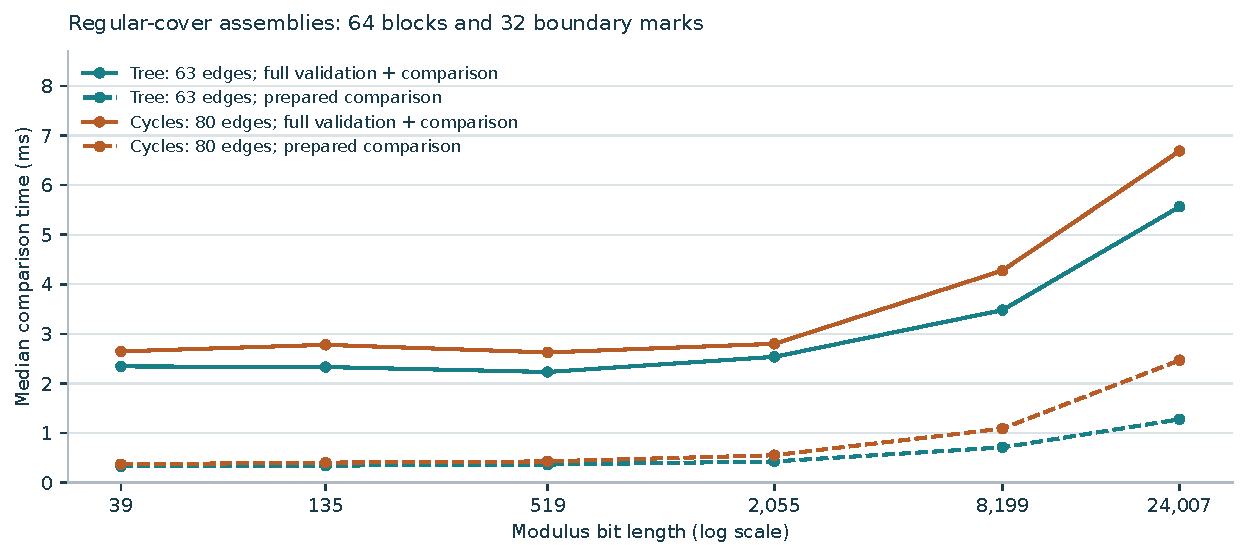
\includegraphics[width=\textwidth]{figures/gluing_scaling.pdf}
\caption{Observed gluing times as the binary modulus grows. Lines connect
measured medians and are not fitted complexity laws. The same-algorithm
control ratios range from 0.952 to 1.496; the study therefore supports
feasibility on huge encoded degrees, not precise small-factor speed claims.}
\label{fig:gluing}
\end{figure}

The exhaustive oracle is intentionally confined to small degree. There is
no measured expanded baseline at a 24,007-bit modulus, and the article
does not invent one by extrapolation. The proof supplies the reason the
compact computation avoids sheet enumeration.

\subsection{Normal disks: supplied witnesses of exponential weight}

The independent checker accepts every saved Fibonacci fixture from one
through 256 tetrahedra. For comparison, fresh worker processes call
Regina's \code{isCompressingDisc(True)} on the same supplied surfaces.
The flag gives the native predicate the advantage of assuming connectedness;
the independent checker proves it, and also validates the ambient
triangulation. Native process startup, import, and input construction are
excluded from its predicate clock. The native API documentation explicitly
describes cutting and retriangulating, with large-coordinate memory costs
\cite{regina}; this is a comparison against that API, not against the
best known theoretical normal-surface algorithms.

\begin{table}[htbp]
\centering\small
\begin{tabular}{@{}rrrrl@{}}
\toprule
$t$ & Elementary disks $D_t$ & Checker (ms) & Native (ms) & Paired ratio\\
\midrule
6 & 84 & 0.410 & 0.614 & $1.36\times$\\
10 & 605 & 0.782 & 4.924 & $7.06\times$\\
14 & 4,176 & 0.924 & 44.903 & $49.37\times$\\
18 & 28,652 & 1.173 & 414.236 & $353.25\times$\\
22 & 196,413 & 1.689 & -- & 5/5 memory failures\\
32 & 24,157,812 & 2.090 & -- & not attempted\\
64 & $\approx1.177\cdot10^{14}$ & 4.168 & -- & not attempted\\
128 & $\approx2.792\cdot10^{27}$ & 9.778 & -- & not attempted\\
256 & $\approx1.571\cdot10^{48}$ & 24.943 & -- & not attempted\\
\bottomrule
\end{tabular}
\caption{Supplied normal-surface verification, not surface discovery or
diagram-level recognition. Every checker row completes in all five rounds.
The native 22-tetrahedron runs raise MemoryError under the 768 MiB process
address-space cap. Exact large integers are retained in the fixtures.}
\label{tab:normal}
\end{table}

Native workers have a three-second allowance and a 768 MiB address-space
limit. The 22-tetrahedron failures are memory failures, not completed
predicates at the limit. For 256 tetrahedra the maximum coordinate has 178
bits, and the complete serialized input plus certificate is 69,434 bytes.
The interval includes reconstructing the finite manifold, matching,
primitivity, rank, Euler characteristic, and boundary parity. No expansion
proportional to $D_t$ occurs.

\begin{figure}[htbp]
\centering
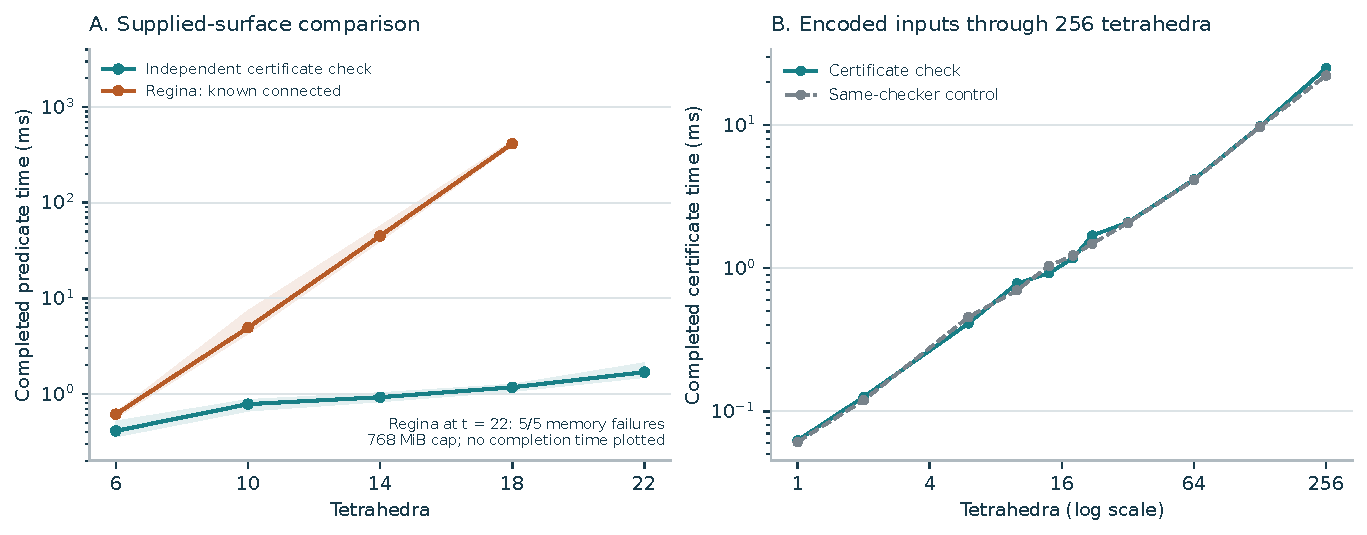
\includegraphics[width=\textwidth]{figures/normal_verification.pdf}
\caption{Normal-disk experiment. Panel A compares completed predicates;
shading is the observed range of five samples, not a confidence interval.
Panel B shows the checker and a same-checker control through the largest
saved input. The proof, rather than a regression fitted to these points,
establishes polynomial dependence on encoded input size.}
\label{fig:normal}
\end{figure}

The independent ambient-manifold audit samples 1,200 finite face-pairing
inputs with one to five tetrahedra. The checker and Regina both accept
58 as connected compact orientable manifolds with one torus boundary,
with zero mismatches. Accepted raw inputs are retained. Twelve native
layered-solid-torus constructions agree with the independent fixture
generator. In addition, 128 single-coordinate mutations are rejected, and
boundary-parallel vertex-linking disks are rejected by the parity condition.
These tests strengthen implementation confidence; the soundness theorem
does not rest on the random sample.

\subsection{Integrated validation and release structure}

The final integrated test run passes all \TestCount{} tests in
\TestSeconds{} seconds, with Regina enabled and no skipped tests.
The complete log is included. The new endpoint,
regular-cover, and normal-disk test modules contain 10, 14, and 12 tests,
respectively; individual tests often perform exhaustive or randomized
comparisons over many inputs. Historical reference implementations needed
by the maintained tests are included in their original relative paths.

Integration also exposed an existing worker-communication defect on the
tested Python runtime. Retrying a timed \code{communicate(None)} could leave
a large partially written stdin payload unsent, causing an otherwise simple
worker to time out. The original 500,000-byte regression reproduced this
failure. The correction makes one public \code{communicate(payload)} call
in an I/O thread while the caller polls cancellation and the absolute
deadline. Cleanup reaps the child, joins that thread, and closes the pipes.
Two additional regressions cover large simultaneous output and cancellation
with blocked input. This compatibility correction does not contribute to
the measured kernel gains, and is identified separately in the patch.

The release contains the complete article source, its compiled PDF, figure
sources and figures, the runnable maintained \code{fast/} code and tests,
the necessary historical test oracles, new fixtures and raw measurements,
an integration note, a patch against the pinned checkout, and a SHA-256
manifest. Generated interpreter caches and unrelated historical benchmark
collections are excluded. The integration patch is checked against the
pinned baseline before packaging.

The three measurement entry points are
\path{fast/benchmark_compressed_endpoint.py},
\path{fast/regular_cover_research/reproduce.py}, and
\path{fast/certificate_research/benchmark.py}.
Figures can be rebuilt from the saved data without rerunning the benchmarks.
The README records commands, optional dependencies, and the exact provenance
of the baseline and archived ablation. This makes each claim independently
inspectable and makes an unsuccessful reproduction report actionable.
